\documentclass{article}
\usepackage[utf8]{inputenc}
\usepackage{amsmath}
\usepackage{setspace}
\usepackage{mathtools}
\usepackage{amssymb}
\usepackage{amsfonts}
\newcommand\der[2]{\frac{\partial{#1}}{\partial{#2}}}
\usepackage{sectsty}
\usepackage[parfill]{parskip}
\usepackage{changepage}   % for the adjustwidth environment
\usepackage{graphicx}
\graphicspath{ {./Pictures/} }
\usepackage{float}
\usepackage[margin=1.25in]{geometry}
\setlength{\parindent}{1.25em}
\sectionfont{\fontsize{12}{12}\selectfont}
\nonfrenchspacing
\renewcommand{\baselinestretch}{1.5}
\usepackage{indentfirst}

\title{Macroeconomics B Notes}
\author{Nicholas Umashev \footnote{Please see google notes}}
\date{2019}

\begin{document}

\maketitle

\section{Dynamic Optimisation in Continuous Time}

\par \underline{Continuous vs Discrete Time}: in discrete time the intervals between periods are $\Delta>0$ (e.g. the interval between $t$ and $t+1$ is 1), in continuous time the intervals between periods are $\Delta \rightarrow 0$
\par \underline{Continuous Variables Issue}: while state variables are often naturally continuous, when using computational methods we can only evaluation the value function  on a finite number of points
\begin{itemize}
    \item \underline{Solution}: we can address this problem via using (1) discretization of the state space, or, (2) polynomial approximation to the value function
\end{itemize}
\par \underline{Discretization Method}: consider a problem with continuous state and control variables $\mathfrak{x} \in \mathbb{R}$, discretization just replaces $\mathfrak{x}$ and $\mathfrak{u}$ by the finite grids $\widehat{\mathfrak{x}} = \{ x^{1}, \dots, x^{n} \}$ and $\widehat{\mathfrak{u}} = \{ u^{1}, \dots, u^{n} \}$
\begin{itemize}
    \item \underline{Value Function Impact}: now the value function becomes a finite list of numbers, $V = [V^{1}, \dots, V^{n}]^{T}$
    \item  \underline{Advantage}: the maximization step is much simpler than under the original bellman equation, which is a key advantage of discretization methods
    \item  \underline{Disadvantage}: there is a "curse of dimensionality" in muiltidimensional state spaces where we must decides whether to have $N$ points for a one-dimensional state space vs $N^{k}$ points for a k-dimensional state space
    \begin{itemize}
        \item  \underline{Grid Decision}: requires some a-priori information about the state space, which is sometimes difficult to obtain (e.g. upper and lower bounds)
    \end{itemize}
    \item  \underline{Optimal Growth Illustration}: suppose $V(k) = \max_{k'} \left\{ \ln (Ak^{\alpha} - k') + \beta V(k') \right\}$ where in this case $\mathfrak{x} = \mathfrak{u}$
    \begin{itemize}
        \item \underline{Discretization}: if we discretize $\mathfrak{x}$ then the Bellman equation becomes $V_{i} = \max_{j} \left\{ \ln (Ak^{\alpha}_{i} - k_{j}) + \beta V_{j} \right\}$ for all $i = 1, \dots, n$
        \item \underline{Value Function Iteration Solution}: suppose we applied value function iteration and therefore iterate on the mapping $V_{i}^{s} = \max \left\{ \ln(Ak^{\alpha}_{i} - k_{1}) + \beta V_{1}^{s-1}, \dots, \ln(Ak_{i}^{\alpha} - k_{n}) + \beta V_{n}^{s-1} \right\}$ for all $i = 1, \dots, n$ where $s$ indexes the iteration step
        \begin{itemize}
            \item 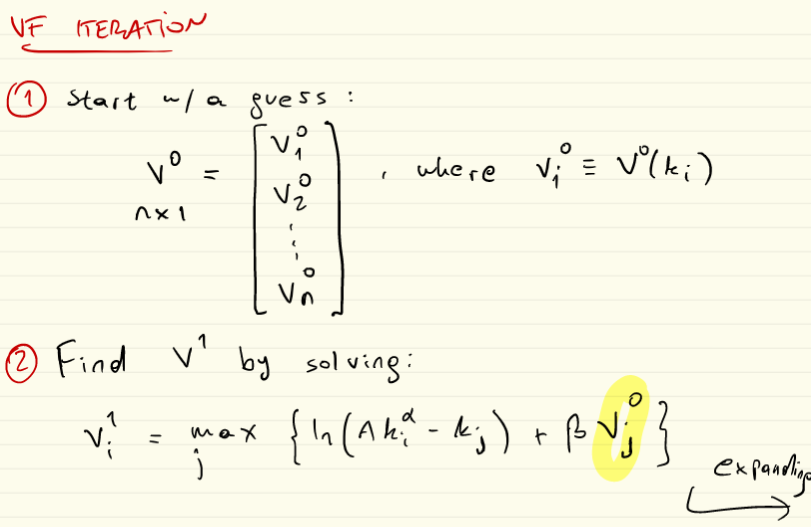
\includegraphics[width=8cm, height=6cm]{pic1}
            \item 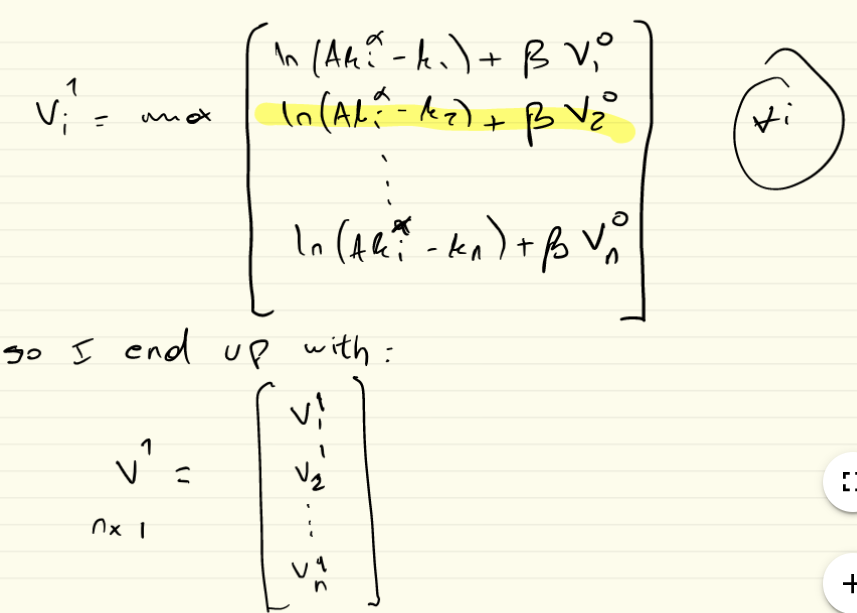
\includegraphics[width=8cm, height=6cm]{pic2}
            \item 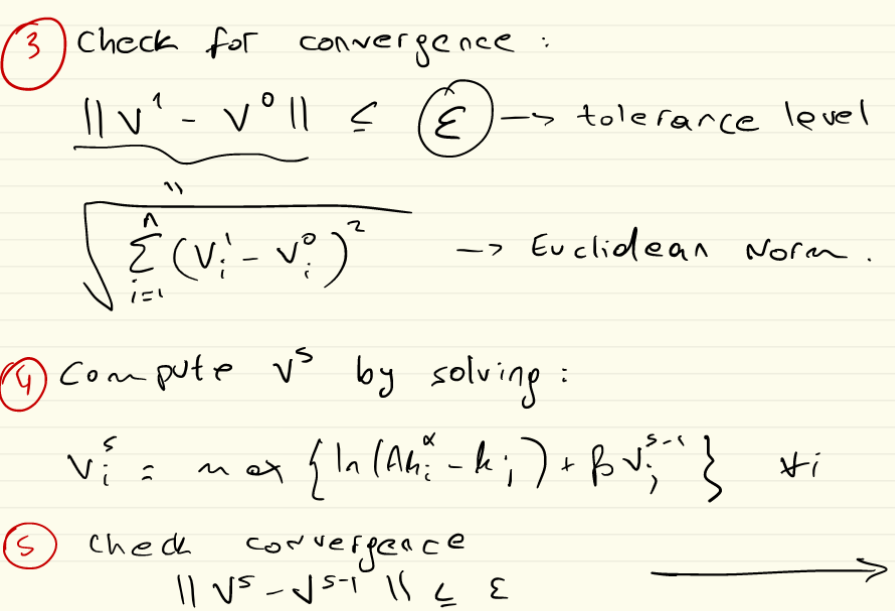
\includegraphics[width=8cm, height=6cm]{pic3}
            \item 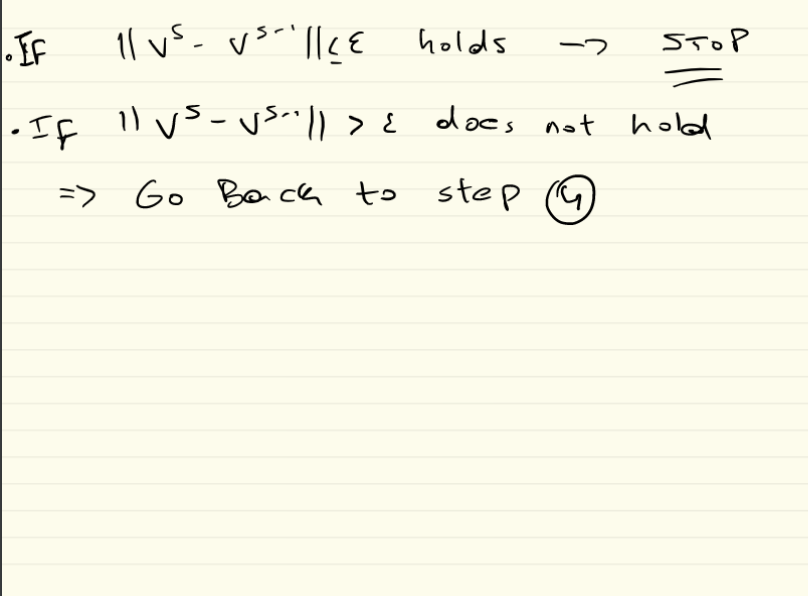
\includegraphics[width=8cm, height=6cm]{pic4}
        \end{itemize}
    \end{itemize}
\end{itemize}
\par \underline{Ordinary Differential Equations (ODEs)}: a "differential" equation" is one where the unknown is a function (instead of a variable) and the equation includes one or more of the derivatives of the function, an "ordinary differential equation" equation is one for which the unknown is a function of only one variable (typically time)
\begin{itemize}
    \item \underline{Partial ODEs}: where the unknown is a function of more than one variable
    \item  \underline{First-Order ODE Form}: $\dot{x}(t) = F(t, x(t))$, where $\dot{x}(t) \equiv dx(t)/dt$ and $t \in [t_{a}, t_{b}]$
    \begin{itemize}
        \item \underline{Unknown}: here the unknown is a function $x(t)$ with $x: [t_{a}, t_{b}] \rightarrow \mathbb{R}$
        \item  \underline{Uniqueness}: the solution is not unique with the form having infinitely many solutions indexed by an integrating constant C. However, generally the constant C can be uniquely determined by requiring the solution to pass through a given point on the $tx$-plane
    \end{itemize}
\end{itemize}

\end{document}
